\chapter{Programmazione dinamica}

\index{programmazione dinamica}

La \key{programmazione dinamica}
è una tecnica che combina la correttezza della
ricerca completa con l'efficienza degli algoritmi
greedy.
La programmazione dinamica può essere
applicata nei casi in cui il problema da risolvere
può essere suddiviso in sottoproblemi
parzialmente sovrapposti e che possono
essere risolti in maniera indipendente.
La programmazione dinamica può essere utilizzata
in due casi:

\begin{itemize}
\item
\key{Trovare una soluzione ottimale}:
si vuole trovare una soluzione che è la
più grande o la più piccola possibile.
\item
\key{Contare il numero di soluzioni}:
si vuole calcolare il numero totale di 
soluzioni possibili.
\end{itemize}

Si vedrà prima come usare la programmazione
dinamica per trovare la soluzione ottima di un problema,
e poi la stessa idea verrà utilizzata per 
contare le soluzioni.

Comprendere come utilizzare la programmazione dinamica
è un momento cruciale nella carriera di ogni
programmatore che dedideri partecipare a delle gare algoritmiche.
Nonostante l'idea di base sia semplice,
la difficoltà risiede in come applicarla
in problemi anche molto differenti tra di loro.
Questo capitolo introduce un insieme di problemi classici 
che sono un buon punto di partenza.

\section{Problema delle monete}

Questo primo problema era già stato studiato 
nel capitolo 6: dato un insieme di monete di valori
$\texttt{coins} = \{c_1,c_2,\ldots,c_k\}$,
si vuole ottenere una somma
$n$ che utilizzi il minor numero di monete possibile.

Nel capitolo 6 il problema è stato risolto utilizzando
un algoritmo greedy che ad ogni passo sceglie 
la moneta più grande possibile.
L'algoritmo greedy funziona ad esempio se i valori delle
monete sono quelli degli euro,
ma nel caso generale con valori delle monete qualsiasi
non è detto produca il risultato ottimo.

Adesso si vedrà che utilizzando la
programmazione dinamica il problema 
potrà essere risolto in modo efficiente,
garantendo il risultato corretto 
per insiemi qualsiasi dei valori delle monete.
Questo algoritmo si basa su una formulazione
ricorsiva che esplora tutte le somme possibili,
come nell'approcio a forza bruta.
Però, a differenza di quest'ultimo, la versione
dinamica utilizza la \emph{memoizzazione} e calcola
la risposta a ogni sottoproblema una volta soltanto.

\subsubsection{Formulazione ricorsiva}

L'idea nella programmazione dinamica è quella di 
formulare il problema in forma ricorsiva
in modo che il problema possa essere 
risolto combinando le soluzioni di sottoproblemi
più piccoli.
Nel problema delle monete una formulazione
ricorsiva del problema è la seguente:
qual è il più piccolo numero di monete richiesto per 
formare una somma $x$?

Sia $\texttt{solve}(x)$
il minimo numero di monete richieste per 
formare una somma $x$. Il valore
della funzione dipende dai valori delle monete
che si hanno a disposizione.
Avendo come insieme $\texttt{coins} = \{1,3,4\}$,
i primi valori della funzione saranno:

\[
\begin{array}{lcl}
\texttt{solve}(0) & = & 0 \\
\texttt{solve}(1) & = & 1 \\
\texttt{solve}(2) & = & 2 \\
\texttt{solve}(3) & = & 1 \\
\texttt{solve}(4) & = & 1 \\
\texttt{solve}(5) & = & 2 \\
\texttt{solve}(6) & = & 2 \\
\texttt{solve}(7) & = & 2 \\
\texttt{solve}(8) & = & 2 \\
\texttt{solve}(9) & = & 3 \\
\texttt{solve}(10) & = & 3 \\
\end{array}
\]

Per esempio, $\texttt{solve}(10)=3$,
poichè servono almeno 3 monete per formare
la somma 10, che in questo caso sono $3+3+4=10$.

La proprietà essenziale delle funzione $\texttt{solve}$ 
è che i suoi valori possono essere calcolati
ricorsivamente a partire da valori più piccoli.

L'idea è di focalizzarsi sulla \emph{prima}
moneta che può essere scelta per la somma.
Nell'esempio mostrato la prima moneta 
potrebbe essere 1, 3 o 4.
Scegliendo come prima moneta quella di valore 1,
il problema diventa come formare la somma 9
usando il minor numero di monete,
che, come si vede, è un sottoproblema del problema originale.
Ovviamente lo stesso discorso si potrebbe applicare
alle monete di valore 3 e 4.
Quindi ne deriva la seguente formula ricorsiva per
il calcolo del minimo numero di monete:
\begin{equation*}
\begin{split}
\texttt{solve}(x) = \min( & \texttt{solve}(x-1)+1, \\
                           & \texttt{solve}(x-3)+1, \\
                           & \texttt{solve}(x-4)+1).
\end{split}
\end{equation*}
Il caso base della ricorsione è $\texttt{solve}(0)=0$,
perchè per formare la somma 0 non sono necessarie monete.
Per esempio
\[ \texttt{solve}(10) = \texttt{solve}(7)+1 = \texttt{solve}(4)+2 = \texttt{solve}(0)+3 = 3.\]

Una volta compreso il meccanismo è possibile dare una forma
generale alla funzione ricorsiva che calcola il minimo
numero di monete necessarie a formare una somma $x$:
\begin{equation*}
    \texttt{solve}(x) = \begin{cases}
               \infty               & x < 0\\
               0               & x = 0\\
               \min_{c \in \texttt{coins}} \texttt{solve}(x-c)+1 & x > 0 \\
           \end{cases}
\end{equation*}

Se $x<0$, il valore è $\infty$,
poichè è impossibile creare una somma negativa
a partire da monete di valore positivo.
Se invece $x=0$, il valore è $0$,
poichè, come detto in precedenza,
non sono necessarie monete per formare
una somma vuota.
Infine, se $x>0$,
la variabile $c$, che rappresenta la prima moneta scelta,
assume tutti i valori possibili 
delle monete e verrà poi scelta ricorsivamente 
quella che minimizza il numero di monete.

Una volta definita la funzione ricorsiva che risolve il problema,
può essere direttamente implementata in C++
(la costante \texttt{INF} rappresenta l'infinito):

\begin{lstlisting}
int solve(int x) {
    if (x < 0) return INF;
    if (x == 0) return 0;
    int best = INF;
    for (auto c : coins) {
        best = min(best, solve(x-c)+1);
    }
    return best;
}
\end{lstlisting}

Comunque, implementata in questo modo,
la funzione non è efficiente,
poichè c'è un numero esponenziale
di modi di costruire questa somma.
Si vedrà adesso come renderla efficiente
utilizzando una tecnica chiamata \emph{memoizzazione}\footnote{Per il lettore italiano: 
il termine memoizzazione non va confuso con memorizzazione. Nell'originale inglese non c'è
questo pericolo perchè i due termini vengono resi con \emph{memoization} e \emph{store}, nella 
traduzione italiana è stata usata \emph{memoizzazione} per 
riferirsi alla tecnica e \emph{memorizzazione} quando un
valore viene memorizzato in memoria.}.

\subsubsection{Usare la memoizzazione}

\index{memoizzazione}

L'idea base della programmazione dinamica è quella
di usare la \key{memoizzazione} 
per calcolare i valori di una funzione ricorsiva
in maniera efficiente.
Questo si ottiene memorizzando i valori della funzione
in un array (eventualmente multidimensionale) dopo che sono stati calcolati la prima volta.
In questo modo, per ogni parametro, il valore della funzione viene calcolato
ricorsivamente una sola volta, dopodichè può essere
recuperato dall'array.

Nel problema delle monete si potrebbero utilizzare
questi due array:

\begin{lstlisting}
bool ready[N];
int value[N];
\end{lstlisting}

dove $\texttt{ready}[x]$ indica se il valore di
$\texttt{solve}(x)$ è stato calcolato,
e se lo è $\texttt{value}[x]$
ne contiene il valore.
La costante $N$ deve essere scelta in modo tale
che gli array possano contenere tutti i valori necessari.

A questo punto un'implementazione efficiente
può essere scritta in questo modo:

\begin{lstlisting}
int solve(int x) {
    if (x < 0) return INF;
    if (x == 0) return 0;
    if (ready[x]) return value[x];
    int best = INF;
    for (auto c : coins) {
        best = min(best, solve(x-c)+1);
    }
    value[x] = best;
    ready[x] = true;
    return best;
}
\end{lstlisting}

I casi base $x<0$ e $x=0$ sono gestiti come prima,
poi la funzione controlla attraverso il valore di 
$\texttt{ready}[x]$ se
$\texttt{solve}(x)$ già stato calcolato in precedenza
e memorizzato in $\texttt{value}[x]$ e se lo è
viene direttamente ritornato.
Altrimenti la funzione calcola il valore
$\texttt{solve}(x)$ ricorsivamente e lo memorizza 
in $\texttt{value}[x]$.

In questo modo la funzione diventa efficiente,
poichè la risposta per ogni valore del parametro $x$
è calcolata ricorsivamente una volta soltanto e successivamente
quel valore può essere recuperato in $O(1)$ attraverso
l'utilizzo dell'array $\texttt{value}$.
La complessità computazionale dell'algoritmo diventa quindi $O(nk)$,
dove $n$ è la somma da ottenere e $k$ è il numero di monete.

Si può notare che sarebbe possibile 
costruire l'array \texttt{value} \emph{iterativamente}
usando un ciclo che semplicemente calcola tutti i 
valori di $\texttt{solve}$ per i parametri $0 \ldots n$:
\begin{lstlisting}
value[0] = 0;
for (int x = 1; x <= n; x++) {
    value[x] = INF;
    for (auto c : coins) {
        if (x-c >= 0) {
            value[x] = min(value[x], value[x-c]+1);
        }
    }
}
\end{lstlisting}

Nelle competizioni di alto livello, i programmatori
più abili preferiscono questa seconda implementazione,
poichè è più corta da scrivere e ha dei costi costanti più bassi
(pur avendo la stessa complessità computazionale),
quindi nei prossimi esempi verrà usata
questa tipo di implementazione ricorsiva.
Comunque è spesso più semplice applicare
la programmazione dinamica partendo 
da una funzione ricorsiva.

\subsubsection{Costruzione di una soluzione}

In alcuni problemi può essere richiesto sia
di trovare il valore della soluzione ottima
che di mostrare un modo per ottenere quella soluzione.

Nel problema delle monete, ad esempio, è possibile
dichiarare un altro array che indica per ogni
somma di monete la prima moneta che appartiene a 
una soluzione ottimale:
\begin{lstlisting}
int first[N];
\end{lstlisting}
L'algoritmo può quindi essere modificato nel seguente modo:
\begin{lstlisting}
value[0] = 0;
for (int x = 1; x <= n; x++) {
    value[x] = INF;
    for (auto c : coins) {
        if (x-c >= 0 && value[x-c]+1 < value[x]) {
            value[x] = value[x-c]+1;
            first[x] = c;
        }
    }
}
\end{lstlisting}
Facendo così e utilizzando il vettore \textit{first}, è
possibile stampare le monete che appaiono in una soluzione ottima
per la somma $x$:
\begin{lstlisting}
while (n > 0) {
    cout << first[n] << "\n";
    n -= first[n];
}
\end{lstlisting}

\subsubsection{Contare il numero di soluzioni}

Si consideri un'altra versione del problema delle monete,
nella quale lo scopo sia quello di calcolare
il numero totale di modi in cui possa essere 
ottenuta la somma $n$ usando le monete date.
Per esempio, se $\texttt{coins}=\{1,3,4\}$ e
$x=5$, ci sono in totale 6 differenti modi per ottenere la somma richiesta:

\begin{multicols}{2}
\begin{itemize}
\item $1+1+1+1+1$
\item $1+1+3$
\item $1+3+1$
\item $3+1+1$
\item $1+4$
\item $4+1$
\end{itemize}
\end{multicols}

Anche in questo caso il problema può essere risolto ricorsivamente.
Sia $\texttt{solve}(x)$ il numero di modi differenti in cui può
essere formata la somma $x$.
Nell'esempio precedente in cui $\texttt{coins}=\{1,3,4\}$,
allora $\texttt{solve}(5)=6$ e la formula ricorsiva risulta essere:
\begin{equation*}
\begin{split}
\texttt{solve}(x) = & \texttt{solve}(x-1) + \\
                    & \texttt{solve}(x-3) + \\
                    & \texttt{solve}(x-4)  .
\end{split}
\end{equation*}

Quindi la versione generale di questa formula diventa:
\begin{equation*}
    \texttt{solve}(x) = \begin{cases}
               0               & x < 0\\
               1               & x = 0\\
               \sum_{c \in \texttt{coins}} \texttt{solve}(x-c) & x > 0 \\
           \end{cases}
\end{equation*}

Se $x<0$, allora il valore è 0, perchè non ci sono soluzioni.
Se $x=0$, il valore è 1 perchè esiste un solo modo 
per creare la somma vuota.
Altrimenti bisogna calcolare la somma di tutti i valori
della forma $\texttt{solve}(x-c)$ con $c$ contenuto in \texttt{coins}.

Il seguente codice costruisce un array
$\texttt{count}$ tale che
$\texttt{count}[x]$ sia uguale al valore di $\texttt{solve}(x)$
per $0 \le x \le n$:

\begin{lstlisting}
count[0] = 1;
for (int x = 1; x <= n; x++) {
    for (auto c : coins) {
        if (x-c >= 0) {
            count[x] += count[x-c];
        }
    }
}
\end{lstlisting}

Spesso il numero di soluzioni è talmente grande
che non viene richiesto di calcolare il numero esatto, 
ma semplicemente di dare la risposta modulo $m$,
con $m$ ad esempio uguale a $10^9+7$.
Per ottenere questo risultato è sufficiente 
cambiare il codice in modo che tutti i calcoli siano fatti modulo $m$.
Quindi basta aggiungere la linea
\begin{lstlisting}
        count[x] %= m;
\end{lstlisting}
dopo la linea
\begin{lstlisting}
        count[x] += count[x-c];
\end{lstlisting}

Fino a questo punto sono state discusse tutte 
le idee base della programmazione dinamica.
Siccome la programmazione dinamica può essere
usata in un range molto ampio di problemi,
verranno adesso mostrati degli esempi classici,
in modo da comprenderne meglio il funzionamento.

\section{La più lunga sottosequenza crescente}

\index{più lunga sottosequenza crescente}

Il primo problema che verrà esposto è 
quello di trovare la \key{più lunga sottosequenza crescente}
all'interno di un array di $n$ elementi.
Tale sottosequenza è quella con più
elementi, non necessariamente consecutivi, da sinistra a destra,
in cui ogni elemento è più grande del precedente.
Per esempio, nell'array

\begin{center}
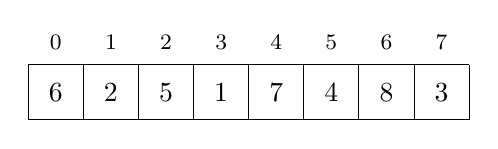
\begin{tikzpicture}[scale=0.7]
\draw (0,0) grid (8,1);
\node at (0.5,0.5) {$6$};
\node at (1.5,0.5) {$2$};
\node at (2.5,0.5) {$5$};
\node at (3.5,0.5) {$1$};
\node at (4.5,0.5) {$7$};
\node at (5.5,0.5) {$4$};
\node at (6.5,0.5) {$8$};
\node at (7.5,0.5) {$3$};

\footnotesize
\node at (0.5,1.4) {$0$};
\node at (1.5,1.4) {$1$};
\node at (2.5,1.4) {$2$};
\node at (3.5,1.4) {$3$};
\node at (4.5,1.4) {$4$};
\node at (5.5,1.4) {$5$};
\node at (6.5,1.4) {$6$};
\node at (7.5,1.4) {$7$};
\end{tikzpicture}
\end{center}
la più lunga sottosequenza crescente 
contiene 4 elementi:
\begin{center}
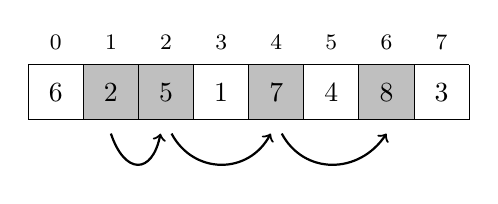
\begin{tikzpicture}[scale=0.7]
\fill[color=lightgray] (1,0) rectangle (2,1);
\fill[color=lightgray] (2,0) rectangle (3,1);
\fill[color=lightgray] (4,0) rectangle (5,1);
\fill[color=lightgray] (6,0) rectangle (7,1);
\draw (0,0) grid (8,1);
\node at (0.5,0.5) {$6$};
\node at (1.5,0.5) {$2$};
\node at (2.5,0.5) {$5$};
\node at (3.5,0.5) {$1$};
\node at (4.5,0.5) {$7$};
\node at (5.5,0.5) {$4$};
\node at (6.5,0.5) {$8$};
\node at (7.5,0.5) {$3$};

\draw[thick,->] (1.5,-0.25) .. controls (1.75,-1.00) and (2.25,-1.00) .. (2.4,-0.25);
\draw[thick,->] (2.6,-0.25) .. controls (3.0,-1.00) and (4.0,-1.00) .. (4.4,-0.25);
\draw[thick,->] (4.6,-0.25) .. controls (5.0,-1.00) and (6.0,-1.00) .. (6.5,-0.25);

\footnotesize
\node at (0.5,1.4) {$0$};
\node at (1.5,1.4) {$1$};
\node at (2.5,1.4) {$2$};
\node at (3.5,1.4) {$3$};
\node at (4.5,1.4) {$4$};
\node at (5.5,1.4) {$5$};
\node at (6.5,1.4) {$6$};
\node at (7.5,1.4) {$7$};
\end{tikzpicture}
\end{center}

Sia $\texttt{length}(k)$ la lunghezza della
più lunga sottosequenza che termina in posizione $k$.
Quindi calcolando tutti i valori di
$\texttt{length}(k)$ con $0 \le k \le n-1$,
si troverà la lunghezza della più lunga sottosequenza
per il vettore di lunghezza $n$.
Ad esempio, i valori di questa funzione 
per l'array visto in precedenza sono i seguenti:
\[
\begin{array}{lcl}
\texttt{length}(0) & = & 1 \\
\texttt{length}(1) & = & 1 \\
\texttt{length}(2) & = & 2 \\
\texttt{length}(3) & = & 1 \\
\texttt{length}(4) & = & 3 \\
\texttt{length}(5) & = & 2 \\
\texttt{length}(6) & = & 4 \\
\texttt{length}(7) & = & 2 \\
\end{array}
\]

Considerando ad esempio il caso $\texttt{length}(6)=4$,
il valore risulta 4 poichè la più lunga sottosequenza che
finisce alla posizione 6 consiste di 4 elementi. Invece per il caso $k=5$
è 2 perchè la più lunga sottosequenza che finisce in posizione 5 può essere
solo {2, 4} oppure {1, 4}, che sono entrambe di lunghezza 2.

Per calcolare il valore di $\texttt{length}(k)$,
è necessario trovare una posizione $i<k$
per la quale $\texttt{array}[i]<\texttt{array}[k]$
e $\texttt{length}(i)$ abbia il maggior valore possibile.
A questo punto il valore di $\texttt{length}(k)$ 
sarà $\texttt{length}(k)=\texttt{length}(i)+1$,
poichè questo è il modo ottimale di aggiungere
$\texttt{array}[k]$ alla sottosequenza.
Se invece non fosse possibile trovare una posizione $i$
per cui valgano le condizioni descritte in precedenza,
allora sarà $\texttt{length}(k)=1$,
il che significa che la sequenza contiene solo
$\texttt{array}[k]$.

Dal momento che tutti i valori della funzione possono essere
calcolati a partire da valori più piccoli,
è possibile usare la programmazione dinamica.
Nel codice seguente i valori della funzione
vengono memorizzati nell'array
$\texttt{length}$.

\begin{lstlisting}
for (int k = 0; k < n; k++) {
    length[k] = 1;
    for (int i = 0; i < k; i++) {
        if (array[i] < array[k]) {
            length[k] = max(length[k],length[i]+1);
        }
    }
}
\end{lstlisting}

Questo algoritmo è di classe $O(n^2)$,
poichè è composto da due cicli annidati.
Si può comunque verificare che è possibile 
implementarlo in modo più efficiente, 
riducendolo a un algoritmo di complessità $O(n \log n)$.
Viene lasciato al lettore come esercizio di trovare il modo di farlo.

\section{Percorsi in una griglia}

Il prossimo problema è di trovare un percorso
in una griglia $n \times n$, che parta dall'angolo in alto 
a sinistra e si concluda nell'angolo in basso 
a destra, avendo la possibilità di muoversi solo
verso il basso e verso destra.
Ogni quadrato della griglia contiene un intero positivo,
e il percorso deve essere costruito in modo
che la somma dei valori dei quadrati che lo 
compongono sia la più grande possibile.

Questa figura mostra un percorso ottimale:

\begin{center}
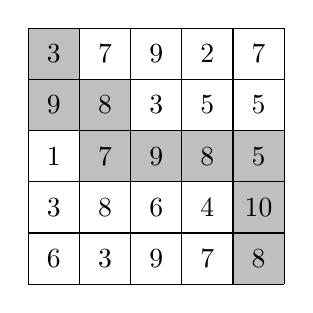
\begin{tikzpicture}[scale=.65]
  \begin{scope}
    \fill [color=lightgray] (0, 9) rectangle (1, 8);
    \fill [color=lightgray] (0, 8) rectangle (1, 7);
    \fill [color=lightgray] (1, 8) rectangle (2, 7);
    \fill [color=lightgray] (1, 7) rectangle (2, 6);
    \fill [color=lightgray] (2, 7) rectangle (3, 6);
    \fill [color=lightgray] (3, 7) rectangle (4, 6);
    \fill [color=lightgray] (4, 7) rectangle (5, 6);
    \fill [color=lightgray] (4, 6) rectangle (5, 5);
    \fill [color=lightgray] (4, 5) rectangle (5, 4);
    \draw (0, 4) grid (5, 9);
    \node at (0.5,8.5) {3};
    \node at (1.5,8.5) {7};
    \node at (2.5,8.5) {9};
    \node at (3.5,8.5) {2};
    \node at (4.5,8.5) {7};
    \node at (0.5,7.5) {9};
    \node at (1.5,7.5) {8};
    \node at (2.5,7.5) {3};
    \node at (3.5,7.5) {5};
    \node at (4.5,7.5) {5};
    \node at (0.5,6.5) {1};
    \node at (1.5,6.5) {7};
    \node at (2.5,6.5) {9};
    \node at (3.5,6.5) {8};
    \node at (4.5,6.5) {5};
    \node at (0.5,5.5) {3};
    \node at (1.5,5.5) {8};
    \node at (2.5,5.5) {6};
    \node at (3.5,5.5) {4};
    \node at (4.5,5.5) {10};
    \node at (0.5,4.5) {6};
    \node at (1.5,4.5) {3};
    \node at (2.5,4.5) {9};
    \node at (3.5,4.5) {7};
    \node at (4.5,4.5) {8};
  \end{scope}
\end{tikzpicture}
\end{center}
La somma dei valori di questo percorso è 67,
che il valore più grande che si può ottenere
costruendo un percorso dall'angolo in alto a sinistra
all'angolo in basso a destra.
Si assuma che le righe e le colonne siano numerate
da 1 a $n$, e $\texttt{value}[y][x]$ sia il valore del quadrato in 
posizione $(y,x)$.
Sia inoltre $\texttt{sum}(y,x)$ la somma massima
di un percorso dall'angolo in alto a destra
fino al quadrato in posizione $(y,x)$.
Allora $\texttt{sum}(n,n)$ sarà la somma 
massima cercata.
Per esempio, nella griglia mostrata sopra,
$\texttt{sum}(5,5)=67$.

La somma può essere ricorsivamente calcolata in questo modo:

\[ \texttt{sum}(y,x) = \max(\texttt{sum}(y,x-1),\texttt{sum}(y-1,x))+\texttt{value}[y][x]\]

Questa formulazione ricorsiva è basata sull'osservazione 
che un percorso che finisce al quadrato $(y,x)$
può arrivare o dal quadrato $(y,x-1)$
o da quello $(y-1,x)$:
\begin{center}
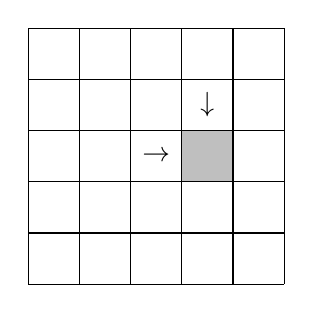
\begin{tikzpicture}[scale=.65]
  \begin{scope}
    \fill [color=lightgray] (3, 7) rectangle (4, 6);
    \draw (0, 4) grid (5, 9);
    
    \node at (2.5,6.5) {$\rightarrow$};
    \node at (3.5,7.5) {$\downarrow$};
    
  \end{scope}
\end{tikzpicture}
\end{center}

Quindi deve essere selezionata la direzione che massimizza
la somma.
Assumendo che $\texttt{sum}(y,x)=0$
se $y=0$ oppure $x=0$ (poichè in tal caso non esiste un percorso),
la formula ricorsiva può essere calcolata per tutte le 
coordinate in cui $y=1$ oppure $x=1$.

Dal momento che la funzione \texttt{sum} ha due parametri,
l'array di supporto alla programmazione dinamica avrà due
dimensioni.
Per esempio, usando la matrice
\begin{lstlisting}
int sum[N][N];
\end{lstlisting}
il calcolo della somma sarà il seguente:
\begin{lstlisting}
for (int y = 1; y <= n; y++) {
    for (int x = 1; x <= n; x++) {
        sum[y][x] = max(sum[y][x-1],sum[y-1][x])+value[y][x];
    }
}
\end{lstlisting}
La complessità computazionale di questo algoritmo sarà quindi $O(n^2)$.

\section{I problemi dello zaino}

\index{knapsack}
\index{zaino}

Il termine \key{knapsack}(zaino in italiano, come verrà chiamato nel seguito)
fa riferimento a una varietà di problemi
nei quali viene dato un insieme di oggetti
e bisogna trovare un sottoinsieme
che soddisfi certe proprietà.
I "problemi dello zaino" possono essere
spesso risolti usando la programmazione dinamica.

In questa sezione il problema analizzato
è il seguente: data una lista di pesi
$[w_1,w_2,\ldots,w_n]$,
determinare tutte le somme che possono essere 
costruite usando quei pesi.
Per esempio, se i pesi fossero
$[1,3,3,5]$, si otterrebbero le seguenti somme:

\begin{center}
\begin{tabular}{rrrrrrrrrrrrr}
 0 & 1 & 2 & 3 & 4 & 5 & 6 & 7 & 8 & 9 & 10 & 11 & 12 \\
\hline
 X & X & & X & X & X & X & X & X & X & & X & X \\
\end{tabular}
\end{center}

Come si può vedere è possibile costruire tutte le somme
tra $0 \ldots 12$ tranne 2 e 10.
Ad esempio, la somma 7 si può ottenere selezionando
i pesi $[1,3,3]$.

Per risolvere questo problema, è sufficiente
risolvere i sottoproblemi in cui vengono usati solo i primi
$k$ pesi per costruire le somme.
Sia $\texttt{possible}(x,k)=\textrm{true}$ se è
possibile costruire la somma $x$ usando i primi $k$ pesi,
altrimenti $\texttt{possible}(x,k)=\textrm{false}$.
I valori di questa funzione possono essere calcolati 
ricorsivamente in questo modo:
\[ \texttt{possible}(x,k) = \texttt{possible}(x-w_k,k-1) \lor \texttt{possible}(x,k-1) \]
La formula si basa sul fatto che è possibile 
usare o meno il peso $w_k$ per costruire una somma.
Se viene usato il peso $w_k$, il problema si riduce a formare 
la somma $x-w_k$ usando i primi $k-1$ pesi,
se invece non viene usato, allora bisogna formare la somma $x$
sempre con i primi $k-1$ pesi.
I casi base sono i seguenti,
\begin{equation*}
    \texttt{possible}(x,0) = \begin{cases}
               \textrm{true}    & x = 0\\
               \textrm{false}   & x \neq 0 \\
           \end{cases}
\end{equation*}
poichè, se non viene usato nessun peso,
è possibile formare solo la somma di valore 0.

La seguente tabella mostra tutti i valori della funzione
per i pesi $[1,3,3,5]$, dove il simbolo ''X'' indica 
i valori per i quali la funzione è true:

\begin{center}
\begin{tabular}{r|rrrrrrrrrrrrr}
$k \backslash x$ & 0 & 1 & 2 & 3 & 4 & 5 & 6 & 7 & 8 & 9 & 10 & 11 & 12 \\
\hline
 0 & X & \\
 1 & X & X \\
 2 & X & X & & X & X \\
 3 & X & X & & X & X & & X & X \\
 4 & X & X & & X & X & X & X & X & X & X & & X & X \\
\end{tabular}
\end{center}

Dopo aver calcolato questi valori, $\texttt{possible}(x,n)$
indica quali somme possono essere costruite usando tutti gli \emph{n} pesi.

Sia $W$ la somma totale dei pesi.
Allora la seguente soluzione
che sfrutta la programmazione dinamica per
implementare la funzione ricorsiva in maniera
efficiente, avrà un costo di tipo $O(nW)$:
\begin{lstlisting}
possible[0][0] = true;
for (int k = 1; k <= n; k++) {
    for (int x = 0; x <= W; x++) {
        if (x-w[k] >= 0) possible[x][k] |= possible[x-w[k]][k-1];
        possible[x][k] |= possible[x][k-1];
    }
}
\end{lstlisting}

Comunque è anche possibile scrivere un'implementazione
che usa solo un array monodimensionale $\texttt{possible}[x]$
che indica se è possibile costruire un sottoinsieme di somma $x$.
Il trucco consiste nell'aggiornare l'array da destra verso sinistra
per ogni nuovo peso:
\begin{lstlisting}
possible[0] = true;
for (int k = 1; k <= n; k++) {
    for (int x = W; x >= 0; x--) {
        if (possible[x]) possible[x+w[k]] = true;
    }
}
\end{lstlisting}

Va notato che l'idea generale presentata qui può
essere applicata a molti problemi dello zaino.
Per esempio, se ogni oggetto è contraddistinto da un peso e da un valore,
è possibile determinare per ogni somma dei pesi la massima
somma dei valori.

\section{Distanza di edit (edit distance)}

\index{edit distance}
\index{Levenshtein distance}
\index{distanza di edit}
\index{Distanza di Levenshtein}


La \key{distanza di edit}(edit distance) o \key{Distanza di Levenshtein}\footnote{Questa distanza prende il 
nome da V. I. Levenshtein, che ne studio la relazione con i codici binari\cite{lev66}.}
è il numero minimo di operazioni di editing
che sono necessarie per trasformare una stringa in un'altra stringa.
Le operazioni di editing permesse sono le seguenti:
\begin{itemize}
\item inserimento di un carattere (e.g. \texttt{ABC} $\rightarrow$ \texttt{ABCA})
\item rimozione di un carattere (e.g. \texttt{ABC} $\rightarrow$ \texttt{AC})
\item modifica di un carattere (e.g. \texttt{ABC} $\rightarrow$ \texttt{ADC})
\end{itemize}

Per esempio la distanza di edit tra
\texttt{LOVE} e \texttt{MOVIE} è 2,
perchè basta prima fare
 \texttt{LOVE} $\rightarrow$ \texttt{MOVE}
(modifica) e poi
\texttt{MOVE} $\rightarrow$ \texttt{MOVIE}
(inserimento).
Questo è il più piccolo numero possibile di operazioni,
perchè è evidente che una sola operazione non è sufficiente.

Sia data la stringa \texttt{x}
di lunghezza $n$ e una stringa \texttt{y} di lunghezza $m$,
e si voglia calcolare la distanza di edit tra
\texttt{x} e \texttt{y}.
Per risolvere il problema si definisca la funzione
$\texttt{distance}(a,b)$ che calcola la distanza di edit
tra i prefissi
$\texttt{x}[0 \ldots a]$ e $\texttt{y}[0 \ldots b]$.
Utilizzando questa funzione la distanza di edit
tra \texttt{x} e \texttt{y} risulterà uguale a $\texttt{distance}(n-1,m-1)$.

I valori di \texttt{distance} possono essere calcolati nel seguente modo:
\begin{equation*}
\begin{split}
\texttt{distance}(a,b) = \min(& \texttt{distance}(a,b-1)+1, \\
                           & \texttt{distance}(a-1,b)+1, \\
                           & \texttt{distance}(a-1,b-1)+\texttt{cost}(a,b)).
\end{split}
\end{equation*}
dove $\texttt{cost}(a,b)=0$ se $\texttt{x}[a]=\texttt{y}[b]$,
altrimenti $\texttt{cost}(a,b)=1$.
Questa formula considera che la stringa \texttt{x} possa
esse editata nei seguenti modi:
\begin{itemize}
\item $\texttt{distance}(a,b-1)$: inserisce un carattere alla fine di \texttt{x}
\item $\texttt{distance}(a-1,b)$: rimuove l'ultimo carattere da \texttt{x}
\item $\texttt{distance}(a-1,b-1)$: verifica se l'ultimo carattere di \texttt{x} è uguale all'ultimo di \texttt{x},
altrimenti lo modifica per renderlo uguale 
\end{itemize}
Nei primi due casi è necessaria un'operazione di editing
(inserimento o rimozione).
Nell'ultimo caso, se $\texttt{x}[a]=\texttt{y}[b]$,
non serve nessuna operazione di editing, 
altrimenti sarà necessaria un'operazione di editing (modifica).

La seguente tabella mostra i valori di \texttt{distance}
per il caso di esempio:
\begin{center}
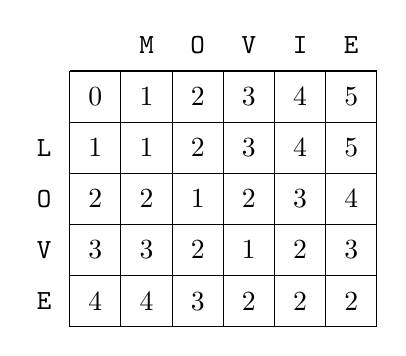
\begin{tikzpicture}[scale=.65]
  \begin{scope}
    %\fill [color=lightgray] (5, -3) rectangle (6, -4);
    \draw (1, -1) grid (7, -6);
    
    \node at (0.5,-2.5) {\texttt{L}};
    \node at (0.5,-3.5) {\texttt{O}};
    \node at (0.5,-4.5) {\texttt{V}};
    \node at (0.5,-5.5) {\texttt{E}};

    \node at (2.5,-0.5) {\texttt{M}};
    \node at (3.5,-0.5) {\texttt{O}};
    \node at (4.5,-0.5) {\texttt{V}};
    \node at (5.5,-0.5) {\texttt{I}};
    \node at (6.5,-0.5) {\texttt{E}};

    \node at (1.5,-1.5) {$0$};
    \node at (1.5,-2.5) {$1$};
    \node at (1.5,-3.5) {$2$};
    \node at (1.5,-4.5) {$3$};
    \node at (1.5,-5.5) {$4$};
    \node at (2.5,-1.5) {$1$};
    \node at (2.5,-2.5) {$1$};
    \node at (2.5,-3.5) {$2$};
    \node at (2.5,-4.5) {$3$};
    \node at (2.5,-5.5) {$4$};
    \node at (3.5,-1.5) {$2$};
    \node at (3.5,-2.5) {$2$};
    \node at (3.5,-3.5) {$1$};
    \node at (3.5,-4.5) {$2$};
    \node at (3.5,-5.5) {$3$};
    \node at (4.5,-1.5) {$3$};
    \node at (4.5,-2.5) {$3$};
    \node at (4.5,-3.5) {$2$};
    \node at (4.5,-4.5) {$1$};
    \node at (4.5,-5.5) {$2$};
    \node at (5.5,-1.5) {$4$};
    \node at (5.5,-2.5) {$4$};
    \node at (5.5,-3.5) {$3$};
    \node at (5.5,-4.5) {$2$};
    \node at (5.5,-5.5) {$2$};
    \node at (6.5,-1.5) {$5$};
    \node at (6.5,-2.5) {$5$};
    \node at (6.5,-3.5) {$4$};
    \node at (6.5,-4.5) {$3$};
    \node at (6.5,-5.5) {$2$};
  \end{scope}
\end{tikzpicture}
\end{center}

Nell'angolo in basso a destra delle tabella
si trova il valore della distanza di edit tra
\texttt{LOVE} e \texttt{MOVIE}, che, come detto in precedenza, è 2.
Questa tabella mostra anche come costruire
la più corta sequenza di operazioni di editing.
In questo caso il percorso è il seguente:

\begin{center}
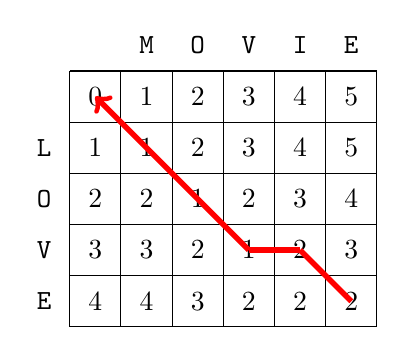
\begin{tikzpicture}[scale=.65]
  \begin{scope}
    \draw (1, -1) grid (7, -6);
    
    \node at (0.5,-2.5) {\texttt{L}};
    \node at (0.5,-3.5) {\texttt{O}};
    \node at (0.5,-4.5) {\texttt{V}};
    \node at (0.5,-5.5) {\texttt{E}};

    \node at (2.5,-0.5) {\texttt{M}};
    \node at (3.5,-0.5) {\texttt{O}};
    \node at (4.5,-0.5) {\texttt{V}};
    \node at (5.5,-0.5) {\texttt{I}};
    \node at (6.5,-0.5) {\texttt{E}};

    \node at (1.5,-1.5) {$0$};
    \node at (1.5,-2.5) {$1$};
    \node at (1.5,-3.5) {$2$};
    \node at (1.5,-4.5) {$3$};
    \node at (1.5,-5.5) {$4$};
    \node at (2.5,-1.5) {$1$};
    \node at (2.5,-2.5) {$1$};
    \node at (2.5,-3.5) {$2$};
    \node at (2.5,-4.5) {$3$};
    \node at (2.5,-5.5) {$4$};
    \node at (3.5,-1.5) {$2$};
    \node at (3.5,-2.5) {$2$};
    \node at (3.5,-3.5) {$1$};
    \node at (3.5,-4.5) {$2$};
    \node at (3.5,-5.5) {$3$};
    \node at (4.5,-1.5) {$3$};
    \node at (4.5,-2.5) {$3$};
    \node at (4.5,-3.5) {$2$};
    \node at (4.5,-4.5) {$1$};
    \node at (4.5,-5.5) {$2$};
    \node at (5.5,-1.5) {$4$};
    \node at (5.5,-2.5) {$4$};
    \node at (5.5,-3.5) {$3$};
    \node at (5.5,-4.5) {$2$};
    \node at (5.5,-5.5) {$2$};
    \node at (6.5,-1.5) {$5$};
    \node at (6.5,-2.5) {$5$};
    \node at (6.5,-3.5) {$4$};
    \node at (6.5,-4.5) {$3$};
    \node at (6.5,-5.5) {$2$};

    \path[draw=red,thick,-,line width=2pt] (6.5,-5.5) -- (5.5,-4.5);
    \path[draw=red,thick,-,line width=2pt] (5.5,-4.5) -- (4.5,-4.5);
    \path[draw=red,thick,->,line width=2pt] (4.5,-4.5) -- (1.5,-1.5);
  \end{scope}
\end{tikzpicture}
\end{center}

Gli ultimi caratteri di \texttt{LOVE} e \texttt{MOVIE}
sono uguali, quindi la distanza di edit tra di loro 
è uguale alla distanza di edit tra \texttt{LOV} e \texttt{MOVI}.
Usando un'operazione di editing è possibile 
rimuovere il carattere \texttt{I} da \texttt{MOVI}.
A questo punto la distanza è maggiore di un'unità rispetto alla
distanza di edit tra \texttt{LOV} e \texttt{MOV}, e proseguendo in questo modo si arriva
all'angolo in alto a sinistra.

\section{Contare le pavimentazioni}

A volte gli stati della soluzione di un problema di 
programmazione dinamica sono più complessi di 
una semplice combinazione di numeri.
Si consideri, ad esempio, il problema
di calcolate in quanti modi distinti 
possa essere completamente riempita
(pavimentato) una griglia $n \times m$ 
usando delle piastrelle di dimensione $1 \times 2$ e $2 \times 1$.
Per esempio una soluzione valida per una griglia $4 \times 7$ è
la seguente:
\begin{center}
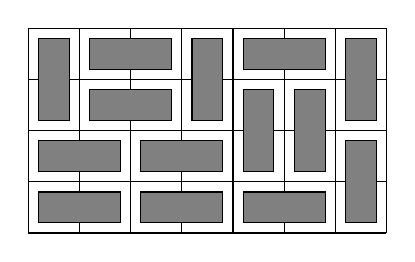
\begin{tikzpicture}[scale=.65]
    \draw (0,0) grid (7,4);
    \draw[fill=gray] (0+0.2,0+0.2) rectangle (2-0.2,1-0.2);
    \draw[fill=gray] (2+0.2,0+0.2) rectangle (4-0.2,1-0.2);
    \draw[fill=gray] (4+0.2,0+0.2) rectangle (6-0.2,1-0.2);
    \draw[fill=gray] (0+0.2,1+0.2) rectangle (2-0.2,2-0.2);
    \draw[fill=gray] (2+0.2,1+0.2) rectangle (4-0.2,2-0.2);
    \draw[fill=gray] (1+0.2,2+0.2) rectangle (3-0.2,3-0.2);
    \draw[fill=gray] (1+0.2,3+0.2) rectangle (3-0.2,4-0.2);
    \draw[fill=gray] (4+0.2,3+0.2) rectangle (6-0.2,4-0.2);

    \draw[fill=gray] (0+0.2,2+0.2) rectangle (1-0.2,4-0.2);
    \draw[fill=gray] (3+0.2,2+0.2) rectangle (4-0.2,4-0.2);
    \draw[fill=gray] (6+0.2,2+0.2) rectangle (7-0.2,4-0.2);
    \draw[fill=gray] (4+0.2,1+0.2) rectangle (5-0.2,3-0.2);
    \draw[fill=gray] (5+0.2,1+0.2) rectangle (6-0.2,3-0.2);
    \draw[fill=gray] (6+0.2,0+0.2) rectangle (7-0.2,2-0.2);

\end{tikzpicture}
\end{center}
e il numero totale di soluzioni è 781.

Il problema può essere risolto usando la programmazione dinamica e
attraversando la griglia riga per riga.
Ogni riga in una soluzione può essere rappresentata
come una stringa che contiene $m$ caratteri appartenenti a questo insieme: 
$\{\sqcap, \sqcup, \sqsubset, \sqsupset \}$.
Per esempio, la soluzione mostrata sopra consiste di 4 righe 
che corrispondono alle seguenti stringhe:
\begin{itemize}
\item
$\sqcap \sqsubset \sqsupset \sqcap \sqsubset \sqsupset \sqcap$
\item
$\sqcup \sqsubset \sqsupset \sqcup \sqcap \sqcap \sqcup$
\item
$\sqsubset \sqsupset \sqsubset \sqsupset \sqcup \sqcup \sqcap$ 
\item
$\sqsubset \sqsupset \sqsubset \sqsupset \sqsubset \sqsupset \sqcup$
\end{itemize}

Sia $\texttt{count}(k,x)$ il numero di modi in cui può essere
costruita una soluzione considerando le righe $1 \ldots k$
in una griglia in modo che la stringa $x$ corrisponda alla riga $k$.

È possibile usare la programmazione dinamica poichè
lo stato di una riga dipende solo dallo stato della riga precedente.

Una soluzione è valida se la riga $1$ non contiene il carattere $\sqcup$,
la riga $n$ non contiene il carattere $\sqcap$,
e tutte le righe consecutive sono \emph{compatibili}.
Per esempio, le righe
$\sqcup \sqsubset \sqsupset \sqcup \sqcap \sqcap \sqcup$ e
$\sqsubset \sqsupset \sqsubset \sqsupset \sqcup \sqcup \sqcap$ 
sono compatibili, mentre le righe
$\sqcap \sqsubset \sqsupset \sqcap \sqsubset \sqsupset \sqcap$ e
$\sqsubset \sqsupset \sqsubset \sqsupset \sqsubset \sqsupset \sqcup$
non sono compatibili.

Dal momento che una riga consiste di esattamente $m$ caratteri 
e ci sono quattro scelte per ogni carattere, il numero di
righe distinte è $4^m$.
Quindi la complessità di questo algoritmo è
$O(n 4^{2m})$ poichè è necessario iterare attraverso tutti gli
$O(4^m)$ stati possibili di ogni riga, e, per ogni stato,
si sono $O(4^m)$ stati possibili per la riga precedente.
In pratica è una buona idea ruotare la griglia in modo 
che il lato più corto abbia lunghezza $m$,
poichè il fattore $4^{2m}$ è dominante per quanto riguarda il tempo di esecuzione.

È inoltre possibile rendere la soluzione ancora più efficiente
usando una rappresentazione più compatta per le righe.
Si può facilmente verificare che è sufficiente sapere
quali colonne della riga precedente contengono la parte superiore
di una piastrella verticale.
Risulta quindi possibile rappresentare una riga usando solo i caratteri
$\sqcap$ e $\Box$, dove $\Box$ è una combinazione di caratteri
$\sqcup$, $\sqsubset$ e $\sqsupset$.
Usando questa rappresentazione, ci sono solo
$2^m$ righe distinte e la complessità totale diventa 
$O(n 2^{2m})$.

Come osservazione finale, è curioso notare che esiste una formula diretta
che calcola il numero di pavimentazioni diverse\footnote{
Ancora più sorprendentemente, questa formula è stata scoperta nel 1961 da due team di ricerca \cite{kas61,tem61} in maniera 
indipendente.}:
\[ \prod_{a=1}^{\lceil n/2 \rceil} \prod_{b=1}^{\lceil m/2 \rceil} 4 \cdot (\cos^2 \frac{\pi a}{n + 1} + \cos^2 \frac{\pi b}{m+1})\]
Questa formula è molto efficiente, perchè calcola il numero 
di pavimentazioni in tempo $O(nm)$,
ma dal momento che la risposta è il prodotto di numeri reali,
il problema è quello di come memorizzare in maniera
accurata i passaggi intermedi.
